\begin{figure}[H]
    \centering
    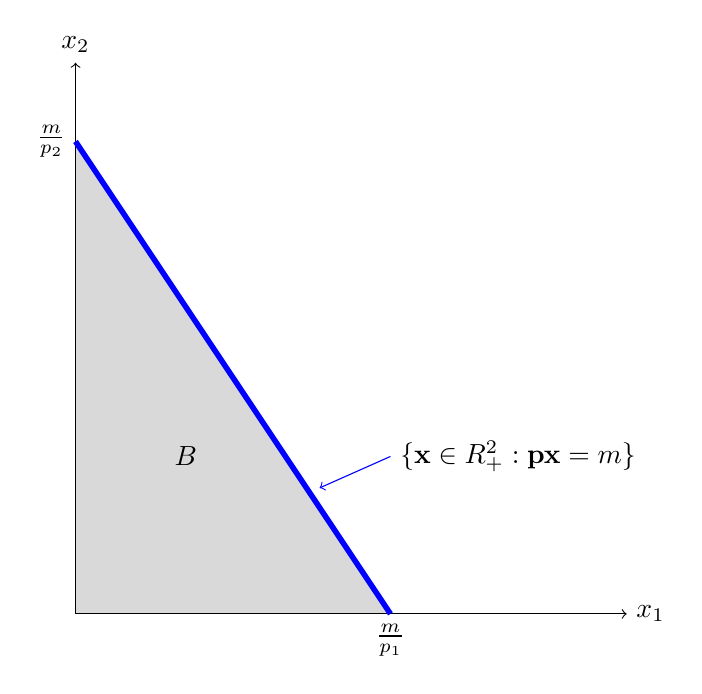
\begin{tikzpicture}[scale=2.0]
        \path[fill=gray!30] (2,0)-- (0,0)-- (0,3)-- cycle;
        \node at (0.7,1) {$B$};
        \draw[->] (0, 0) -- (3.5, 0) node[right] {$x_1$};
        \draw[->] (0, 0) -- (0, 3.5) node[above] {$x_2$};
        \node[below] at (2,0) {$\frac{m}{p_1}$};
        \node[left] at (0,3) {$\frac{m}{p_2}$};
        \draw[domain=0:2, variable=\x, blue, line width=2pt] plot ({\x}, {-3/2 * \x + 3});
        \draw[blue,->] (2,1) -- (1.55,0.8);
        \node[right] at (2,1) {$\{\mathbf{x} \in \mathbbm{R}_{+}^2: \mathbf{px} = m\}$};
    \end{tikzpicture}
\end{figure}